\section*{\hfill{}УСЛОВИЕ\hfill{}}
В пекарню приходят клиенты каждые $4\pm1$ минуты. Обслуживание на кассе просиходит $3\pm2$ минуты. Если в очередь на кассу содержит больше 5 человек, то клиент уходит. С вероятностью 10\% клиента не заинтересует ассортимент и он уйдет; 30\%~--- клиент закажет уже готовую продукцию, что приведёт к выдаче; 5\%~--- продукцию, которую по тем или иным причинам приготовить не представляется возможным, что приведёт к уходу клиента; 35\%~--- клиент закажет продукцию, которую будет необходимо и возможно приготовить. Заказ клиента с 60\% вероятностью будет маленьким, а с вероятностью 40\%~--- большим. Повар 1 и повар 2 занимаются только маленькими заказами, а повар 3~--- только большими. Время приготовления продукции каждым поваром составляет $10\pm2$ минут, $11\pm2$ минут и $20\pm4$ минут соотвественно. Выбор между поваром 1 и поваром 2 происходит по равномерному распределению. Результат приготовления попадает на выдачу. С вероятностью 5\% продукция на выдаче не понравится клиенту и он уйдёт.

Промоделировать процесс обслуживания 500 клиентов, определить вероятность отказа. Реализовать на GPSS.

\section*{\hspace{1.25cm}1\quad{}Теоретическая часть}
На рисунке\ref{img:concept} изображена структурная схема рассматриваемой концептуальной модели.
\begin{figure}[H]
    \centering
    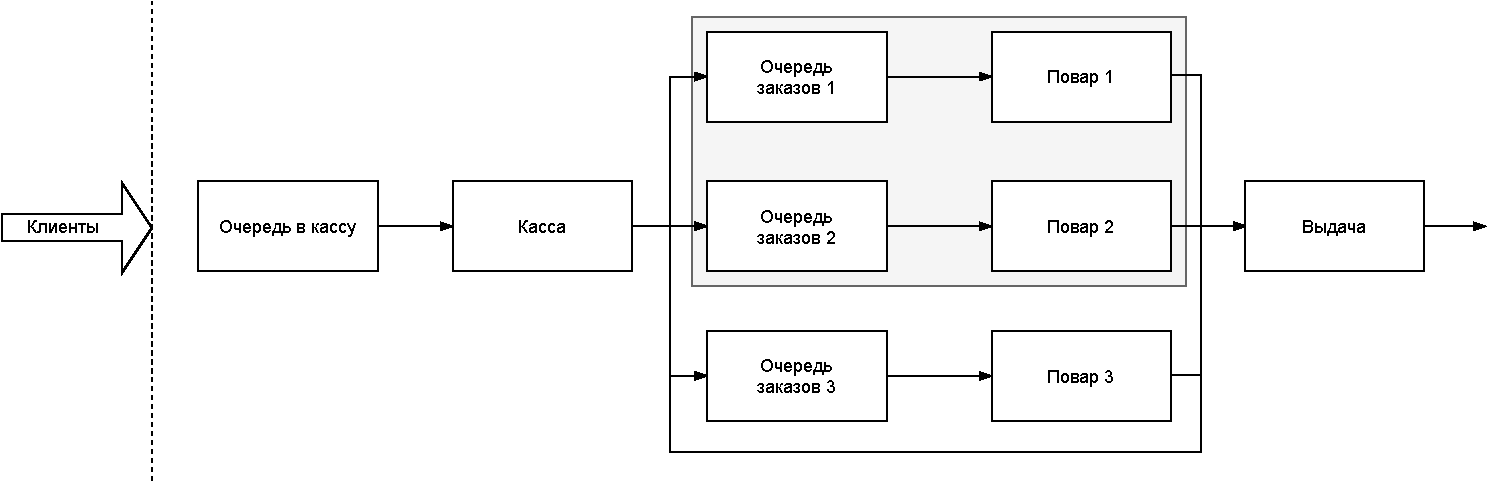
\includegraphics[width=1\textwidth]{pdf/concept.pdf}
    \caption{Структурная схема}
    \label{img:concept}
\end{figure}

\section*{\hspace{1.25cm}2\quad{}Практическая часть}
\begin{lstlisting}[language=c,caption={Листинг}]
GENERATE 4,1,0,500 ; 500 клиентов приходят каждые 4+-1 минуты

			; если в очереди нет места, клиент уходит
L_CASHIER		TEST L	Q$Q_CASHIER,5,L_REFUSAL_Q_CASHIER
			; клиент занимает место в очереди
		QUEUE	Q_CASHIER
			; кассир начинает обслуживание клиента
		SEIZE	D_CASHIER
			; клиент проходит на кассу
		DEPART	Q_CASHIER
			; задержка клиента на кассе
		ADVANCE	3,2
			; обслуживание на кассе завершенно
		RELEASE	D_CASHIER
			; сохранение случайного целого от 0 до 1000
			; в первый параметр транзакта
		ASSIGN	1,RN1
			; сравнение значения параметра
			; со значением функции распределения
			; * 1000
		TEST G	P1,100,L_REFUSAL_D_CASHIER_1
		TEST G	P1,500,L_DELIVERY
		TEST G	P1,550,L_REFUSAL_D_CASHIER_2
		TEST G	P1,685,L_COOK1
		TEST G	P1,820,L_COOK2
		TRANSFER	,L_COOK3,,

			; заказ клиента попадает в очередь к повару
L_COOK1		QUEUE	Q_COOK1
			; повар берёт заказ
		SEIZE	D_COOK1
			; взятый заказ покидает очередь
		DEPART	Q_COOK1
			; задержка на время приготовления
		ADVANCE	10,2
			; повар освобождается
		RELEASE	D_COOK1
			; переход к выдаче
		TRANSFER	,L_DELIVERY,,

; аналогично
L_COOK2		QUEUE	Q_COOK2
		SEIZE	D_COOK2
		DEPART	Q_COOK2
		ADVANCE	11,2
		RELEASE	D_COOK2
		TRANSFER	,L_DELIVERY,,

; аналогично
L_COOK3		QUEUE	Q_COOK3
		SEIZE	D_COOK3
		DEPART	Q_COOK3
		ADVANCE	20,4
		RELEASE	D_COOK3
		TRANSFER	,L_DELIVERY,,

			; заказ попадает в очередь на выдачу
L_DELIVERY	QUEUE	Q_DELIVERY
			; работник пекарни выдаёт заказ
		SEIZE	D_DELIVERY
			; заказ покидает очередь
		DEPART	Q_DELIVERY
			; задержка на время выдачи
		ADVANCE	1,0.25
			; завершение выдачи
		RELEASE	D_DELIVERY
			; клиент забирает заказ или отказывается
		TRANSFER	0.05,L_SUCCESS,L_REFUSAL_D_DELIVERY

L_REFUSAL_Q_CASHIER		TRANSFER ,L_REFUSAL,,
L_REFUSAL_D_CASHIER_1	TRANSFER ,L_REFUSAL,,
L_REFUSAL_D_CASHIER_2	TRANSFER ,L_REFUSAL,,
L_REFUSAL_D_DELIVERY	TRANSFER ,L_REFUSAL,,
L_REFUSAL			TRANSFER ,L_END,,

L_SUCCESS			TRANSFER ,L_END,,

L_END	SAVEVALUE	N_L_REFUSAL_Q_CASHIER,N$L_REFUSAL_Q_CASHIER
	SAVEVALUE	N_L_REFUSAL_D_CASHIER_1,N$L_REFUSAL_D_CASHIER_1
	SAVEVALUE	N_L_REFUSAL_D_CASHIER_2,N$L_REFUSAL_D_CASHIER_2
	SAVEVALUE	N_L_REFUSAL_D_DELIVERY,N$L_REFUSAL_D_DELIVERY
	SAVEVALUE	N_REFUSALS,N$L_REFUSAL
	SAVEVALUE	N_SUCCESSES,N$L_SUCCESS
	SAVEVALUE R_PROBABILITY,(N$L_REFUSAL / (N$L_SUCCESS + N$L_REFUSAL))

TERMINATE 1
START 500
\end{lstlisting}

На рисунке~\ref{img:results} представлены результаты выполнения программы.
\begin{figure}[H]
    \centering
    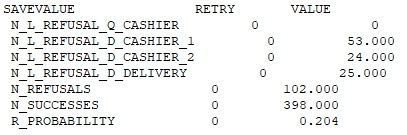
\includegraphics[width=0.6\textwidth]{images/scr01.jpg}
    \caption{Результаты}
    \label{img:results}
\end{figure}

\section*{\hfill{}ВЫВОД\hfill{}}
В настоящей лабораторной работе была промоделирована информационная система, в которую поступают клиенты. Эта система состоит нескольких блоков, а именно: очередь в кассу, касса, три очереди к поварам и три повара, а так же пункт выдачи. Выходными данными являются вероятность отказа и количество клиентов, отказ получивших.
